%\documentclass[border=0cm,convert={outext=.png}]{standalone}
\documentclass[border=0cm]{standalone}
% Documentclass to directly create a PNG-files when invoking 'pdflatex'

\usepackage{xcolor}
\usepackage{tikz}
\usetikzlibrary{arrows.meta}
\renewcommand{\familydefault}{\sfdefault}
\colorlet{ngreen}{green!80!black}
\colorlet{nred}{red!80!black}
\colorlet{ngray}{white!80!black}

\usetikzlibrary{calc}

\usetikzlibrary{fadings}

\makeatletter
\pgfdeclareradialshading{tikz@lib@fade@circle@5}{\pgfpointorigin}{%
	color(0pt)=(pgftransparent!0); color(23.75bp)=(pgftransparent!0);%
	color(25bp)=(pgftransparent!100); color(50bp)=(pgftransparent!100)%
}
\pgfdeclareradialshading{tikz@lib@fade@circle@90}{\pgfpointorigin}{%
	color(0pt)=(pgftransparent!100); color(15bp)=(pgftransparent!100);%
	color(25bp)=(pgftransparent!50); color(50bp)=(pgftransparent!50)%
}
\pgfdeclarefading{circle with fuzzy edge 5 percent}{%
	\pgfuseshading{tikz@lib@fade@circle@15}%
}
\pgfdeclarefading{circle with fuzzy edge 90 percent}{%
	\pgfuseshading{tikz@lib@fade@circle@90}%
}
\makeatother
\begin{tikzfadingfrompicture}[name=custom fade]%
	\path(-0.2cm,0.2cm) rectangle (1.2cm,-2cm); % Arrow line is an overlay!
	\pgfinterruptboundingbox
	\draw[very thick,transparent!20,->] (0cm,0cm) .. controls +(0cm,-1cm) and +(0cm,1cm) .. (1cm,-2cm);
	\endpgfinterruptboundingbox
\end{tikzfadingfrompicture}

\usepackage{pgfplots}
\usepgfplotslibrary{fillbetween}
\usetikzlibrary{fadings}
\tikzfading[name=myfading, right color=transparent!50, left color=transparent!0]


\tikzset{
	autogreen/.style={fill=green!80!black},
	autored/.style={fill=red!80!black},
	sensoryline/.style={line width=0.8,draw=white!50!black,opacity=0.5},
	exsynsensory/.style={-{Triangle[length=0.09cm,width=0.09cm]},line width=0.8,draw=white!50!black,opacity=0.5},
	inhsynsensory/.style={-{Bar[width=0.13cm]},shorten >= 0.1cm,line width=0.8,draw=white!50!black,opacity=0.5},
	exsyn/.style={-{Triangle[length=0.09cm,width=0.09cm]},line width=0.8,looseness=1,draw=white!50!black,opacity=0.5},
	inhsyn/.style={-{Bar[width=0.13cm]},shorten >= 0.1cm,line width=0.8,draw=white!50!black,opacity=0.5,looseness=1},
}

% Load dynamic variables
\definecolor{outputcol}{rgb}{0.2589,0.7937,0.5454}
\definecolor{neur1}{rgb}{0.9769,0.9839,0.0805}
\definecolor{neur2}{rgb}{0.2422,0.1504,0.6603}
\definecolor{neur3}{rgb}{0.2422,0.1504,0.6603}
\definecolor{neur4}{rgb}{0.9749,0.9782,0.0872}
\definecolor{neur5}{rgb}{0.2422,0.1504,0.6603}
\definecolor{neur6}{rgb}{0.9749,0.9782,0.0872}
\definecolor{neur7}{rgb}{0.2422,0.1504,0.6603}
\definecolor{neur8}{rgb}{0.2422,0.1504,0.6603}
\definecolor{neur9}{rgb}{0.9749,0.9782,0.0872}
\definecolor{neur10}{rgb}{0.9749,0.9782,0.0872}
\definecolor{neur11}{rgb}{0.9606,0.7285,0.2312}
\definecolor{neur12}{rgb}{0.2422,0.1504,0.6603}
\definecolor{neur13}{rgb}{0.9749,0.9782,0.0872}
\definecolor{neur14}{rgb}{0.2422,0.1504,0.6603}
\definecolor{neur15}{rgb}{0.2422,0.1504,0.6603}
\definecolor{neur16}{rgb}{0.2422,0.1504,0.6603}
\definecolor{neur17}{rgb}{0.2250,0.4559,0.9985}
\definecolor{neur18}{rgb}{0.8281,0.7481,0.1536}
\definecolor{neur0}{rgb}{0.0770,0.7468,0.7224}
\definecolor{feat0}{rgb}{0.1219,0.6497,0.8862}
\definecolor{feat1}{rgb}{0.8804,0.7372,0.1650}
\definecolor{feat2}{rgb}{0.1778,0.5349,0.9641}
\definecolor{feat3}{rgb}{0.2422,0.1504,0.6603}
\definecolor{feat4}{rgb}{0.2422,0.1504,0.6603}
\definecolor{feat5}{rgb}{0.2422,0.1504,0.6603}
\definecolor{feat6}{rgb}{0.0713,0.6938,0.8409}
\definecolor{feat7}{rgb}{0.1649,0.5755,0.9323}
\definecolor{feat8}{rgb}{0.0770,0.7468,0.7224}
\definecolor{feat9}{rgb}{0.1492,0.5997,0.9147}
\definecolor{feat10}{rgb}{0.1288,0.6408,0.8910}
\definecolor{feat11}{rgb}{0.2422,0.1504,0.6603}
\definecolor{feat12}{rgb}{0.9906,0.8095,0.1906}
\definecolor{feat13}{rgb}{0.0770,0.7468,0.7224}
\definecolor{feat14}{rgb}{0.2422,0.1504,0.6603}
\definecolor{feat15}{rgb}{0.9769,0.9839,0.0805}
\definecolor{feat16}{rgb}{0.0046,0.7301,0.7688}
\definecolor{feat17}{rgb}{0.1755,0.5554,0.9473}
\definecolor{feat18}{rgb}{0.9272,0.7298,0.1973}
\definecolor{feat19}{rgb}{0.1288,0.6408,0.8910}
\definecolor{feat20}{rgb}{0.3671,0.8021,0.4563}
\definecolor{feat21}{rgb}{0.0253,0.7376,0.7492}
\definecolor{feat22}{rgb}{0.1219,0.6497,0.8862}
\definecolor{feat23}{rgb}{0.9440,0.7285,0.2151}
\definecolor{feat24}{rgb}{0.1741,0.7678,0.6527}
\definecolor{feat25}{rgb}{0.9966,0.7740,0.2138}
\definecolor{feat26}{rgb}{0.2422,0.1504,0.6603}
\definecolor{feat27}{rgb}{0.9769,0.9839,0.0805}
\definecolor{feat28}{rgb}{0.0770,0.7468,0.7224}
\definecolor{feat29}{rgb}{0.9769,0.9839,0.0805}
\definecolor{feat30}{rgb}{0.2422,0.1504,0.6603}
\definecolor{feat31}{rgb}{0.2422,0.1504,0.6603}
\newcommand{\titletext}{under $\sigma^2$=0.3 pertubation}
\newcommand{\framecamera}{\includegraphics[width=4cm]{/home/mathias/dev/autonomous_driving/exported_replays/wm_test1_var03_2019-07-31-13-46-58/frames/frame_08315.jpg}}
\newcommand{\framesaliency}{\includegraphics[width=4cm]{/home/mathias/dev/autonomous_driving/exported_replays/wm_test1_var03_2019-07-31-13-46-58/saliency_map/frame_08315.png}}
\newcommand{\gpsmap}{\includegraphics[width=1.0cm]{/home/mathias/dev/autonomous_driving/exported_replays/wm_test1_var03_2019-07-31-13-46-58/gps_map/map_08315.png}}
\newcommand{\layera}{\includegraphics[width=1.3cm]{/home/mathias/dev/autonomous_driving/exported_replays/wm_test1_var03_2019-07-31-13-46-58/saliency_aux/frame_08315_layer_0.png}}
\newcommand{\layerb}{\includegraphics[width=1.1.cm]{/home/mathias/dev/autonomous_driving/exported_replays/wm_test1_var03_2019-07-31-13-46-58/saliency_aux/frame_08315_layer_1.png}}
\newcommand{\layerc}{\includegraphics[width=0.9cm]{/home/mathias/dev/autonomous_driving/exported_replays/wm_test1_var03_2019-07-31-13-46-58/saliency_aux/frame_08315_layer_2.png}}
\newcommand{\featimga}{\includegraphics[width=0.9cm]{/home/mathias/dev/autonomous_driving/exported_replays/wm_test1_var03_2019-07-31-13-46-58/saliency_aux/frame_08315_feat_0.png}}
\newcommand{\featimgb}{\includegraphics[width=0.9cm]{/home/mathias/dev/autonomous_driving/exported_replays/wm_test1_var03_2019-07-31-13-46-58/saliency_aux/frame_08315_feat_1.png}}
\newcommand{\featimgc}{\includegraphics[width=0.9cm]{/home/mathias/dev/autonomous_driving/exported_replays/wm_test1_var03_2019-07-31-13-46-58/saliency_aux/frame_08315_feat_2.png}}
\newcommand{\featimgd}{\includegraphics[width=0.9cm]{/home/mathias/dev/autonomous_driving/exported_replays/wm_test1_var03_2019-07-31-13-46-58/saliency_aux/frame_08315_feat_3.png}}
\newcommand{\featimge}{\includegraphics[width=0.9cm]{/home/mathias/dev/autonomous_driving/exported_replays/wm_test1_var03_2019-07-31-13-46-58/saliency_aux/frame_08315_feat_4.png}}
\newcommand{\featimgf}{\includegraphics[width=0.9cm]{/home/mathias/dev/autonomous_driving/exported_replays/wm_test1_var03_2019-07-31-13-46-58/saliency_aux/frame_08315_feat_5.png}}
\newcommand{\featimgg}{\includegraphics[width=0.9cm]{/home/mathias/dev/autonomous_driving/exported_replays/wm_test1_var03_2019-07-31-13-46-58/saliency_aux/frame_08315_feat_6.png}}
\newcommand{\featimgh}{\includegraphics[width=0.9cm]{/home/mathias/dev/autonomous_driving/exported_replays/wm_test1_var03_2019-07-31-13-46-58/saliency_aux/frame_08315_feat_7.png}}
\newcommand{\automode}{Manual}
\tikzset{%
syn1x0/.style={exsyn},
syn1x1/.style={exsyn},
syn1x3/.style={inhsyn},
syn2x0/.style={exsyn},
syn3x0/.style={exsyn},
syn3x5/.style={exsyn},
syn4x0/.style={exsyn},
syn4x3/.style={inhsyn},
syn5x0/.style={inhsyn},
syn5x5/.style={exsyn},
syn6x0/.style={exsyn},
syn6x4/.style={exsyn},
syn7x1/.style={exsyn},
syn7x2/.style={exsyn},
syn7x3/.style={exsyn},
syn7x4/.style={inhsyn},
syn8x2/.style={exsyn},
syn8x3/.style={exsyn},
syn8x5/.style={exsyn},
syn8x6/.style={exsyn},
syn9x2/.style={exsyn},
syn9x4/.style={exsyn},
syn9x5/.style={exsyn},
syn9x6/.style={inhsyn},
syn10x2/.style={exsyn},
syn10x4/.style={exsyn},
syn10x5/.style={exsyn},
syn10x6/.style={exsyn},
syn11x1/.style={exsyn},
syn11x3/.style={exsyn},
syn11x4/.style={exsyn},
syn11x6/.style={exsyn},
syn12x2/.style={exsyn},
syn12x3/.style={exsyn},
syn12x4/.style={inhsyn},
syn12x5/.style={inhsyn},
syn13x1/.style={exsyn},
syn13x2/.style={exsyn},
syn13x3/.style={exsyn},
syn13x5/.style={exsyn},
syn14x1/.style={inhsyn},
syn14x3/.style={inhsyn},
syn14x5/.style={exsyn},
syn14x6/.style={inhsyn},
syn15x1/.style={inhsyn},
syn15x2/.style={exsyn},
syn15x3/.style={exsyn},
syn15x4/.style={exsyn},
syn16x2/.style={inhsyn},
syn16x3/.style={exsyn},
syn16x4/.style={inhsyn},
syn16x6/.style={exsyn},
syn17x1/.style={inhsyn},
syn17x4/.style={exsyn},
syn17x5/.style={exsyn},
syn17x6/.style={exsyn},
syn18x1/.style={exsyn},
syn18x3/.style={exsyn},
syn18x5/.style={inhsyn},
syn18x6/.style={inhsyn},
sensyn0x7/.style={exsynsensory},
sensyn0x10/.style={exsynsensory},
sensyn0x11/.style={inhsynsensory},
sensyn0x13/.style={exsynsensory},
sensyn0x16/.style={exsynsensory},
sensyn0x17/.style={exsynsensory},
sensyn1x8/.style={exsynsensory},
sensyn1x10/.style={exsynsensory},
sensyn1x13/.style={exsynsensory},
sensyn1x14/.style={inhsynsensory},
sensyn1x15/.style={inhsynsensory},
sensyn1x16/.style={inhsynsensory},
sensyn2x8/.style={inhsynsensory},
sensyn2x10/.style={exsynsensory},
sensyn2x13/.style={inhsynsensory},
sensyn2x16/.style={exsynsensory},
sensyn2x17/.style={inhsynsensory},
sensyn2x18/.style={exsynsensory},
sensyn3x7/.style={exsynsensory},
sensyn3x10/.style={exsynsensory},
sensyn3x12/.style={inhsynsensory},
sensyn3x13/.style={exsynsensory},
sensyn3x16/.style={exsynsensory},
sensyn3x17/.style={exsynsensory},
sensyn4x7/.style={exsynsensory},
sensyn4x8/.style={exsynsensory},
sensyn4x10/.style={exsynsensory},
sensyn4x15/.style={exsynsensory},
sensyn4x17/.style={exsynsensory},
sensyn4x18/.style={inhsynsensory},
sensyn5x9/.style={exsynsensory},
sensyn5x13/.style={exsynsensory},
sensyn5x15/.style={exsynsensory},
sensyn5x16/.style={exsynsensory},
sensyn5x17/.style={inhsynsensory},
sensyn5x18/.style={inhsynsensory},
sensyn6x7/.style={exsynsensory},
sensyn6x9/.style={inhsynsensory},
sensyn6x10/.style={exsynsensory},
sensyn6x11/.style={exsynsensory},
sensyn6x15/.style={inhsynsensory},
sensyn6x16/.style={exsynsensory},
sensyn7x8/.style={exsynsensory},
sensyn7x9/.style={exsynsensory},
sensyn7x10/.style={exsynsensory},
sensyn7x14/.style={exsynsensory},
sensyn7x15/.style={inhsynsensory},
sensyn7x17/.style={exsynsensory},
sensyn8x11/.style={exsynsensory},
sensyn8x12/.style={exsynsensory},
sensyn8x13/.style={exsynsensory},
sensyn8x14/.style={exsynsensory},
sensyn8x16/.style={inhsynsensory},
sensyn8x17/.style={exsynsensory},
sensyn9x8/.style={exsynsensory},
sensyn9x9/.style={exsynsensory},
sensyn9x10/.style={exsynsensory},
sensyn9x11/.style={exsynsensory},
sensyn9x16/.style={exsynsensory},
sensyn9x18/.style={exsynsensory},
sensyn10x7/.style={exsynsensory},
sensyn10x8/.style={exsynsensory},
sensyn10x9/.style={exsynsensory},
sensyn10x10/.style={exsynsensory},
sensyn10x12/.style={exsynsensory},
sensyn10x17/.style={exsynsensory},
sensyn11x7/.style={exsynsensory},
sensyn11x8/.style={exsynsensory},
sensyn11x10/.style={inhsynsensory},
sensyn11x11/.style={inhsynsensory},
sensyn11x15/.style={exsynsensory},
sensyn11x18/.style={exsynsensory},
sensyn12x7/.style={exsynsensory},
sensyn12x10/.style={exsynsensory},
sensyn12x11/.style={exsynsensory},
sensyn12x14/.style={exsynsensory},
sensyn12x15/.style={exsynsensory},
sensyn12x18/.style={exsynsensory},
sensyn13x7/.style={exsynsensory},
sensyn13x9/.style={exsynsensory},
sensyn13x12/.style={exsynsensory},
sensyn13x13/.style={inhsynsensory},
sensyn13x14/.style={inhsynsensory},
sensyn13x16/.style={exsynsensory},
sensyn14x8/.style={inhsynsensory},
sensyn14x10/.style={inhsynsensory},
sensyn14x11/.style={inhsynsensory},
sensyn14x13/.style={exsynsensory},
sensyn14x14/.style={inhsynsensory},
sensyn14x15/.style={exsynsensory},
sensyn15x7/.style={exsynsensory},
sensyn15x9/.style={exsynsensory},
sensyn15x10/.style={inhsynsensory},
sensyn15x11/.style={exsynsensory},
sensyn15x15/.style={exsynsensory},
sensyn15x16/.style={inhsynsensory},
sensyn16x7/.style={exsynsensory},
sensyn16x10/.style={exsynsensory},
sensyn16x12/.style={exsynsensory},
sensyn16x14/.style={exsynsensory},
sensyn16x16/.style={exsynsensory},
sensyn16x17/.style={exsynsensory},
sensyn17x7/.style={inhsynsensory},
sensyn17x9/.style={exsynsensory},
sensyn17x11/.style={exsynsensory},
sensyn17x12/.style={exsynsensory},
sensyn17x13/.style={exsynsensory},
sensyn17x18/.style={exsynsensory},
sensyn18x8/.style={exsynsensory},
sensyn18x9/.style={exsynsensory},
sensyn18x10/.style={exsynsensory},
sensyn18x11/.style={exsynsensory},
sensyn18x14/.style={exsynsensory},
sensyn18x17/.style={exsynsensory},
sensyn19x7/.style={exsynsensory},
sensyn19x8/.style={exsynsensory},
sensyn19x9/.style={inhsynsensory},
sensyn19x12/.style={exsynsensory},
sensyn19x13/.style={exsynsensory},
sensyn19x16/.style={exsynsensory},
sensyn20x9/.style={exsynsensory},
sensyn20x12/.style={exsynsensory},
sensyn20x15/.style={inhsynsensory},
sensyn20x16/.style={exsynsensory},
sensyn20x17/.style={exsynsensory},
sensyn20x18/.style={exsynsensory},
sensyn21x7/.style={exsynsensory},
sensyn21x9/.style={exsynsensory},
sensyn21x10/.style={inhsynsensory},
sensyn21x12/.style={exsynsensory},
sensyn21x15/.style={exsynsensory},
sensyn21x16/.style={exsynsensory},
sensyn22x8/.style={exsynsensory},
sensyn22x9/.style={inhsynsensory},
sensyn22x10/.style={exsynsensory},
sensyn22x13/.style={exsynsensory},
sensyn22x15/.style={exsynsensory},
sensyn22x18/.style={exsynsensory},
sensyn23x7/.style={exsynsensory},
sensyn23x8/.style={exsynsensory},
sensyn23x11/.style={inhsynsensory},
sensyn23x13/.style={exsynsensory},
sensyn23x14/.style={exsynsensory},
sensyn23x17/.style={exsynsensory},
sensyn24x7/.style={exsynsensory},
sensyn24x9/.style={inhsynsensory},
sensyn24x10/.style={exsynsensory},
sensyn24x12/.style={exsynsensory},
sensyn24x17/.style={exsynsensory},
sensyn24x18/.style={inhsynsensory},
sensyn25x7/.style={exsynsensory},
sensyn25x8/.style={exsynsensory},
sensyn25x9/.style={inhsynsensory},
sensyn25x10/.style={exsynsensory},
sensyn25x12/.style={exsynsensory},
sensyn25x17/.style={exsynsensory},
sensyn26x8/.style={exsynsensory},
sensyn26x10/.style={exsynsensory},
sensyn26x14/.style={inhsynsensory},
sensyn26x15/.style={exsynsensory},
sensyn26x16/.style={exsynsensory},
sensyn26x18/.style={inhsynsensory},
sensyn27x7/.style={exsynsensory},
sensyn27x8/.style={exsynsensory},
sensyn27x9/.style={inhsynsensory},
sensyn27x15/.style={exsynsensory},
sensyn27x16/.style={exsynsensory},
sensyn27x17/.style={exsynsensory},
sensyn28x7/.style={exsynsensory},
sensyn28x8/.style={exsynsensory},
sensyn28x11/.style={inhsynsensory},
sensyn28x12/.style={exsynsensory},
sensyn28x13/.style={exsynsensory},
sensyn28x14/.style={inhsynsensory},
sensyn29x7/.style={exsynsensory},
sensyn29x8/.style={exsynsensory},
sensyn29x9/.style={inhsynsensory},
sensyn29x12/.style={exsynsensory},
sensyn29x15/.style={inhsynsensory},
sensyn29x16/.style={exsynsensory},
sensyn30x9/.style={inhsynsensory},
sensyn30x10/.style={inhsynsensory},
sensyn30x11/.style={exsynsensory},
sensyn30x12/.style={exsynsensory},
sensyn30x14/.style={exsynsensory},
sensyn30x18/.style={inhsynsensory},
sensyn31x7/.style={inhsynsensory},
sensyn31x8/.style={exsynsensory},
sensyn31x9/.style={exsynsensory},
sensyn31x13/.style={exsynsensory},
sensyn31x15/.style={inhsynsensory},
sensyn31x16/.style={exsynsensory},
automodecolor/.style={autored},
outputrot/.style={rotate=7.46},
}


\begin{document}
\begin{tikzpicture}[every node/.style={font={\sffamily}},neuron/.style={circle,inner sep=0.07cm,fill=black!40!white},feature/.style={rectangle,minimum width=0.2cm,minimum height=0.1cm,inner sep=0,fill=black!40!white}]


\draw[fill=black] (-2.5,-5.5) rectangle (10.7,2.0);
%\draw[fill=black] (-2.5,-5.5) rectangle (20.5,1.5);
% My Latex code
%\node at (2.5,-2) [opacity=0.25,white,align=center] {\Huge{Work-in }\\\\\\\Huge{progress}};
%\node at (8.5,-2) [opacity=0.25,white,align=center] {\Huge{Do not}\\\\\\\Huge{distribute}};
\node (cam) at (0,-0.2) [inner sep=0,draw=white,line width=1mm] {\framecamera};

\node at (-2.0,1.7) [anchor=west,color=white] {\footnotesize{NCP driving performance}};
\node at (-2.0,1.4) [anchor=west,color=white] {\scriptsize{\titletext}};
\node at (0,0.8) [anchor=center,color=white] {\scriptsize{Camera input stream}};
\node at (0,-3) [anchor=center,color=white] {\scriptsize{Attention map}};

\draw[automodecolor] (-2,-5.30) circle (0.1cm);
\node at (-1.9,-5.30) [anchor=west,color=white] {\scriptsize{Mode:}};
\node at (-1,-5.30) [anchor=west,color=white] {\scriptsize{\automode}};


\node (conv1) at (0,-1.9) [rectangle,draw=olive,line width=1,inner sep=0] {\layera};
\node (conv12) at ($(conv1)+(0.05,-0.05)$) [rectangle,draw=orange,line width=1,inner sep=0] {\layera};
\node (conv13) at ($(conv12)+(0.05,-0.05)$) [rectangle,draw=white,line width=1,inner sep=0] {\layera};

\shade[top color=white!10!black,bottom color=white!50!black] (cam.south east) -- (conv1.north east) -- (conv1.north west) -- (cam.south west) ;

\node (conv2) at (1.5,-1.9) [rectangle,draw=olive,line width=1,inner sep=0] {\layerc};
\node (conv22) at ($(conv2)+(0.05,-0.05)$) [rectangle,draw=orange,line width=1,inner sep=0] {\layerc};
\node (conv23) at ($(conv22)+(0.05,-0.05)$) [rectangle,draw=white,line width=1,inner sep=0] {\layerc};

\node (conv3) at (2.8,-1.8) [rectangle,draw=cyan,line width=1,inner sep=0] {\layerc};
\node (conv32) at ($(conv3)+(0.05,-0.05)$) [rectangle,draw=olive,line width=1,inner sep=0] {\layerc};
\node (conv33) at ($(conv32)+(0.05,-0.05)$) [rectangle,draw=orange,line width=1,inner sep=0] {\layerc};;
\node (conv34) at ($(conv33)+(0.05,-0.05)$) [rectangle,draw=white,line width=1,inner sep=0] {\layerc};

\begin{scope}[shift={(0,-0.1)}]
\node (cfeat7) at (4.2,1) [inner sep=0,rectangle,draw=white,line width=1,minimum width=0.6cm,minimum height=0.3cm,fill=orange!10!gray] {\featimga};
\node (cfeat6) at (4.2,0.2) [inner sep=0,rectangle,draw=white,line width=1,minimum width=0.6cm,minimum height=0.3cm,fill=orange!10!gray] {\featimgb};
\node (cfeat5) at (4.2,-0.6) [inner sep=0,rectangle,draw=white,line width=1,minimum width=0.6cm,minimum height=0.3cm,fill=orange!10!gray] {\featimgc};
\node (cfeat4) at (4.2,-1.4) [inner sep=0,rectangle,draw=white,line width=1,minimum width=0.6cm,minimum height=0.3cm,fill=orange!10!gray] {\featimgd};
\node (cfeat3) at (4.2,-2.2) [inner sep=0,rectangle,draw=white,line width=1,minimum width=0.6cm,minimum height=0.3cm,fill=orange!10!gray] {\featimge};
\node (cfeat2) at (4.2,-3) [inner sep=0,rectangle,draw=white,line width=1,minimum width=0.6cm,minimum height=0.3cm,fill=orange!10!gray] {\featimgf};
\node (cfeat1) at (4.2,-3.8) [inner sep=0,rectangle,draw=white,line width=1,minimum width=0.6cm,minimum height=0.3cm,fill=orange!10!gray] {\featimgg};
\node (cfeat0) at (4.2,-4.6) [inner sep=0,rectangle,draw=white,line width=1,minimum width=0.6cm,minimum height=0.3cm,fill=orange!10!gray] {\featimgh};
\end{scope}


\shade[right color=white!10!black,left color=white!50!black] (conv13.north east) -- (conv2.north west) -- (conv2.south west) -- (conv13.south east) ;
\shade[right color=white!10!black,left color=white!50!black] (conv23.north east) -- (conv3.north west) -- (conv3.south west) -- (conv23.south east) ;
\shade[right color=white!10!black,left color=white!50!black] (conv34.north east) -- (cfeat7.north west) -- (cfeat0.south west) -- (conv34.south east) ;



\node (sal) at (0,-4.0) [,draw=white,line width=1mm,inner sep=0] {\framesaliency};

\begin{scope}[shift={(6.5,0.55)}]
%\node (steer) at (3.5,-2.5) [outputcol,rectangle,draw,minimum width=0.4cm,minimum height=0.4cm] {};
\node (steer) at (3.6,-2.5) [circle,minimum width=0.4cm,minimum height=0.6cm,inner sep=0] {};
\node (n0) at (2.8,-2.5) [neuron,fill=outputcol] {};
\shade[top color=white!10!black,bottom color=white!50!black] (n0.south east) -- (steer.south west) -- (steer.north west) -- (n0.north east) ;

\fill[even odd rule,inner color=outputcol,outer color=black] (3.5,-2.5) circle (0.4);
\draw[thick,color=black] (3.5,-2.5) circle (0.4);
\node (steer) at (3.5,-2.5) [outputrot,circle,inner sep=0] {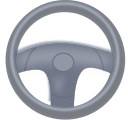
\includegraphics[width=0.7cm]{wheel.png}};
%\draw[thick,red] (3.5,-1.5) arc (0:50:1cm);

\node (n1) at (2.1,-5) [neuron,fill=neur1] {};
\node (n2) at (1.8,-4) [neuron,fill=neur2] {};
\node (n3) at (1.7,-3) [neuron,fill=neur3] {};
\node (n4) at (1.7,-2) [neuron,fill=neur4] {};
\node (n5) at (1.8,-1) [neuron,fill=neur5] {};
\node (n6) at (2.1,0) [neuron,fill=neur6] {};

\node (n7) at (0.9,-5) [neuron,fill=neur7] {};
\node (n8) at (0.5,-4.5) [neuron,fill=neur8] {};
\node (n9) at (0.2,-4.0) [neuron,fill=neur9] {};
\node (n10) at (0.0,-3.5) [neuron,fill=neur10] {};
\node (n11) at (-0.2,-3) [neuron,fill=neur11] {};
\node (n12) at (-0.3,-2.5) [neuron,fill=neur12] {};
\node (n13) at (-0.3,-2.0) [neuron,fill=neur13] {};
\node (n14) at (-0.2,-1.5) [neuron,fill=neur14] {};
\node (n15) at (0.0,-1.0) [neuron,fill=neur15] {};
\node (n16) at (0.2,-0.5) [neuron,fill=neur16] {};
\node (n17) at (0.5,0) [neuron,fill=neur17] {};
\node (n18) at (0.9,0.5) [neuron,fill=neur18] {};
\end{scope}

\begin{scope}[shift={(1,-5)}]
\node (input0) at (4,0.00) [feature,fill=feat0] {};
\node (input1) at (4,0.20) [feature,fill=feat1] {};
\node (input2) at (4,0.40) [feature,fill=feat2] {};
\node (input3) at (4,0.60) [feature,fill=feat3] {};
\node (input4) at (4,0.80) [feature,fill=feat4] {};
\node (input5) at (4,1.00) [feature,fill=feat5] {};
\node (input6) at (4,1.20) [feature,fill=feat6] {};
\node (input7) at (4,1.40) [feature,fill=feat7] {};
\node (input8) at (4,1.60) [feature,fill=feat8] {};
\node (input9) at (4,1.80) [feature,fill=feat9] {};
\node (input10) at (4,2.00) [feature,fill=feat10] {};
\node (input11) at (4,2.20) [feature,fill=feat11] {};
\node (input12) at (4,2.40) [feature,fill=feat12] {};
\node (input13) at (4,2.60) [feature,fill=feat13] {};
\node (input14) at (4,2.80) [feature,fill=feat14] {};
\node (input15) at (4,3.00) [feature,fill=feat15] {};
\node (input16) at (4,3.20) [feature,fill=feat16] {};
\node (input17) at (4,3.40) [feature,fill=feat17] {};
\node (input18) at (4,3.60) [feature,fill=feat18] {};
\node (input19) at (4,3.80) [feature,fill=feat19] {};
\node (input20) at (4,4.00) [feature,fill=feat20] {};
\node (input21) at (4,4.20) [feature,fill=feat21] {};
\node (input22) at (4,4.40) [feature,fill=feat22] {};
\node (input23) at (4,4.60) [feature,fill=feat23] {};
\node (input24) at (4,4.80) [feature,fill=feat24] {};
\node (input25) at (4,5.00) [feature,fill=feat25] {};
\node (input26) at (4,5.20) [feature,fill=feat26] {};
\node (input27) at (4,5.40) [feature,fill=feat27] {};
\node (input28) at (4,5.60) [feature,fill=feat28] {};
\node (input29) at (4,5.80) [feature,fill=feat29] {};
\node (input30) at (4,6.00) [feature,fill=feat30] {};
\node (input31) at (4,6.20) [feature,fill=feat31] {};
\end{scope}

\shade[right color=white!10!black,left color=white!50!black] (cfeat0.north east) -- (input3.north west) -- (input0.south west) -- (cfeat0.south east) ;
\shade[right color=white!10!black,left color=white!50!black] (cfeat1.north east) -- (input7.north west) -- (input4.south west) -- (cfeat1.south east) ;
\shade[right color=white!10!black,left color=white!50!black] (cfeat2.north east) -- (input11.north west) -- (input8.south west) -- (cfeat2.south east) ;
\shade[right color=white!10!black,left color=white!50!black] (cfeat3.north east) -- (input15.north west) -- (input12.south west) -- (cfeat3.south east) ;
\shade[right color=white!10!black,left color=white!50!black] (cfeat4.north east) -- (input19.north west) -- (input16.south west) -- (cfeat4.south east) ;
\shade[right color=white!10!black,left color=white!50!black] (cfeat5.north east) -- (input23.north west) -- (input20.south west) -- (cfeat5.south east) ;
\shade[right color=white!10!black,left color=white!50!black] (cfeat6.north east) -- (input27.north west) -- (input24.south west) -- (cfeat6.south east) ;
\shade[right color=white!10!black,left color=white!50!black] (cfeat7.north east) -- (input31.north west) -- (input28.south west) -- (cfeat7.south east) ;

% Command to motor
\draw[syn1x0] (n1) to[out=20,in=174,looseness=1] (n0);
\draw[syn1x1] (n1) to[out=240,in=300,looseness=7] (n1);
\draw[syn1x3] (n1) to[out=14,in=208,looseness=1] (n3);
\draw[syn2x0] (n2) to[out=-51,in=180,looseness=1] (n0);
\draw[syn3x0] (n3) to[out=28,in=230,looseness=1] (n0);
\draw[syn3x5] (n3) to[out=46,in=202,looseness=1] (n5);
\draw[syn4x0] (n4) to[out=0,in=206,looseness=1] (n0);
\draw[syn4x3] (n4) to[out=0,in=249,looseness=1] (n3);
\draw[syn5x0] (n5) to[out=18,in=152,looseness=1] (n0);
\draw[syn5x5] (n5) to[out=240,in=300,looseness=7] (n5);
\draw[syn6x0] (n6) to[out=-50,in=114,looseness=1] (n0);
\draw[syn6x4] (n6) to[out=51,in=232,looseness=1] (n4);
\draw[syn7x1] (n7) to[out=-8,in=223,looseness=1] (n1);
\draw[syn7x2] (n7) to[out=67,in=185,looseness=1] (n2);
\draw[syn7x3] (n7) to[out=-44,in=208,looseness=1] (n3);
\draw[syn7x4] (n7) to[out=-22,in=190,looseness=1] (n4);
\draw[syn8x2] (n8) to[out=-19,in=179,looseness=1] (n2);
\draw[syn8x3] (n8) to[out=59,in=113,looseness=1] (n3);
\draw[syn8x5] (n8) to[out=69,in=206,looseness=1] (n5);
\draw[syn8x6] (n8) to[out=-32,in=119,looseness=1] (n6);
\draw[syn9x2] (n9) to[out=-32,in=227,looseness=1] (n2);
\draw[syn9x4] (n9) to[out=46,in=204,looseness=1] (n4);
\draw[syn9x5] (n9) to[out=-26,in=146,looseness=1] (n5);
\draw[syn9x6] (n9) to[out=25,in=137,looseness=1] (n6);
\draw[syn10x2] (n10) to[out=15,in=150,looseness=1] (n2);
\draw[syn10x4] (n10) to[out=56,in=133,looseness=1] (n4);
\draw[syn10x5] (n10) to[out=68,in=136,looseness=1] (n5);
\draw[syn10x6] (n10) to[out=0,in=194,looseness=1] (n6);
\draw[syn11x1] (n11) to[out=14,in=235,looseness=1] (n1);
\draw[syn11x3] (n11) to[out=-47,in=180,looseness=1] (n3);
\draw[syn11x4] (n11) to[out=10,in=243,looseness=1] (n4);
\draw[syn11x6] (n11) to[out=-28,in=222,looseness=1] (n6);
\draw[syn12x2] (n12) to[out=-24,in=113,looseness=1] (n2);
\draw[syn12x3] (n12) to[out=-31,in=127,looseness=1] (n3);
\draw[syn12x4] (n12) to[out=47,in=144,looseness=1] (n4);
\draw[syn12x5] (n12) to[out=15,in=226,looseness=1] (n5);
\draw[syn13x1] (n13) to[out=-31,in=134,looseness=1] (n1);
\draw[syn13x2] (n13) to[out=32,in=169,looseness=1] (n2);
\draw[syn13x3] (n13) to[out=13,in=138,looseness=1] (n3);
\draw[syn13x5] (n13) to[out=-41,in=240,looseness=1] (n5);
\draw[syn14x1] (n14) to[out=-62,in=198,looseness=1] (n1);
\draw[syn14x3] (n14) to[out=-1,in=118,looseness=1] (n3);
\draw[syn14x5] (n14) to[out=-11,in=163,looseness=1] (n5);
\draw[syn14x6] (n14) to[out=47,in=213,looseness=1] (n6);
\draw[syn15x1] (n15) to[out=-49,in=151,looseness=1] (n1);
\draw[syn15x2] (n15) to[out=-45,in=211,looseness=1] (n2);
\draw[syn15x3] (n15) to[out=59,in=162,looseness=1] (n3);
\draw[syn15x4] (n15) to[out=65,in=222,looseness=1] (n4);
\draw[syn16x2] (n16) to[out=-12,in=163,looseness=1] (n2);
\draw[syn16x3] (n16) to[out=48,in=119,looseness=1] (n3);
\draw[syn16x4] (n16) to[out=1,in=184,looseness=1] (n4);
\draw[syn16x6] (n16) to[out=-10,in=230,looseness=1] (n6);
\draw[syn17x1] (n17) to[out=60,in=142,looseness=1] (n1);
\draw[syn17x4] (n17) to[out=53,in=120,looseness=1] (n4);
\draw[syn17x5] (n17) to[out=35,in=227,looseness=1] (n5);
\draw[syn17x6] (n17) to[out=18,in=186,looseness=1] (n6);
\draw[syn18x1] (n18) to[out=-69,in=155,looseness=1] (n1);
\draw[syn18x3] (n18) to[out=-15,in=249,looseness=1] (n3);
\draw[syn18x5] (n18) to[out=28,in=199,looseness=1] (n5);
\draw[syn18x6] (n18) to[out=-8,in=220,looseness=1] (n6);
\draw[exsynsensory] ($(n7)-(0.38,-0.32)$) to (n7);
\draw[exsynsensory] ($(n7)-(0.49,-0.12)$) to (n7);
\draw[exsynsensory] ($(n7)-(0.49,0.12)$) to (n7);
\draw[exsynsensory] ($(n7)-(0.38,0.32)$) to (n7);
\draw[exsynsensory] ($(n8)-(0.38,-0.32)$) to (n8);
\draw[inhsynsensory] ($(n8)-(0.49,-0.12)$) to (n8);
\draw[exsynsensory] ($(n8)-(0.49,0.12)$) to (n8);
\draw[exsynsensory] ($(n8)-(0.38,0.32)$) to (n8);
\draw[exsynsensory] ($(n9)-(0.38,-0.32)$) to (n9);
\draw[inhsynsensory] ($(n9)-(0.49,-0.12)$) to (n9);
\draw[exsynsensory] ($(n9)-(0.49,0.12)$) to (n9);
\draw[exsynsensory] ($(n9)-(0.38,0.32)$) to (n9);
\draw[exsynsensory] ($(n10)-(0.38,-0.32)$) to (n10);
\draw[exsynsensory] ($(n10)-(0.49,-0.12)$) to (n10);
\draw[exsynsensory] ($(n10)-(0.49,0.12)$) to (n10);
\draw[exsynsensory] ($(n10)-(0.38,0.32)$) to (n10);
\draw[inhsynsensory] ($(n11)-(0.38,-0.32)$) to (n11);
\draw[exsynsensory] ($(n11)-(0.49,-0.12)$) to (n11);
\draw[exsynsensory] ($(n11)-(0.49,0.12)$) to (n11);
\draw[exsynsensory] ($(n11)-(0.38,0.32)$) to (n11);
\draw[inhsynsensory] ($(n12)-(0.38,-0.32)$) to (n12);
\draw[exsynsensory] ($(n12)-(0.49,-0.12)$) to (n12);
\draw[exsynsensory] ($(n12)-(0.49,0.12)$) to (n12);
\draw[exsynsensory] ($(n12)-(0.38,0.32)$) to (n12);
\draw[exsynsensory] ($(n13)-(0.38,-0.32)$) to (n13);
\draw[exsynsensory] ($(n13)-(0.49,-0.12)$) to (n13);
\draw[inhsynsensory] ($(n13)-(0.49,0.12)$) to (n13);
\draw[exsynsensory] ($(n13)-(0.38,0.32)$) to (n13);
\draw[inhsynsensory] ($(n14)-(0.38,-0.32)$) to (n14);
\draw[exsynsensory] ($(n14)-(0.49,-0.12)$) to (n14);
\draw[exsynsensory] ($(n14)-(0.49,0.12)$) to (n14);
\draw[exsynsensory] ($(n14)-(0.38,0.32)$) to (n14);
\draw[inhsynsensory] ($(n15)-(0.38,-0.32)$) to (n15);
\draw[exsynsensory] ($(n15)-(0.49,-0.12)$) to (n15);
\draw[exsynsensory] ($(n15)-(0.49,0.12)$) to (n15);
\draw[inhsynsensory] ($(n15)-(0.38,0.32)$) to (n15);
\draw[exsynsensory] ($(n16)-(0.38,-0.32)$) to (n16);
\draw[inhsynsensory] ($(n16)-(0.49,-0.12)$) to (n16);
\draw[exsynsensory] ($(n16)-(0.49,0.12)$) to (n16);
\draw[exsynsensory] ($(n16)-(0.38,0.32)$) to (n16);
\draw[exsynsensory] ($(n17)-(0.38,-0.32)$) to (n17);
\draw[inhsynsensory] ($(n17)-(0.49,-0.12)$) to (n17);
\draw[exsynsensory] ($(n17)-(0.49,0.12)$) to (n17);
\draw[exsynsensory] ($(n17)-(0.38,0.32)$) to (n17);
\draw[exsynsensory] ($(n18)-(0.38,-0.32)$) to (n18);
\draw[inhsynsensory] ($(n18)-(0.49,-0.12)$) to (n18);
\draw[inhsynsensory] ($(n18)-(0.49,0.12)$) to (n18);
\draw[exsynsensory] ($(n18)-(0.38,0.32)$) to (n18);
\shade[right color=white!10!black,left color=white!50!black] (input0.north east) -- ($(input0.north east)+(0.78,0.03)$) -- ($(input0.south east)+(0.78,-0.03)$)  -- (input0.south east);
\shade[right color=white!10!black,left color=white!50!black] (input1.north east) -- ($(input1.north east)+(0.75,0.03)$) -- ($(input1.south east)+(0.75,-0.03)$)  -- (input1.south east);
\shade[right color=white!10!black,left color=white!50!black] (input2.north east) -- ($(input2.north east)+(0.73,0.03)$) -- ($(input2.south east)+(0.73,-0.03)$)  -- (input2.south east);
\shade[right color=white!10!black,left color=white!50!black] (input3.north east) -- ($(input3.north east)+(0.70,0.03)$) -- ($(input3.south east)+(0.70,-0.03)$)  -- (input3.south east);
\shade[right color=white!10!black,left color=white!50!black] (input4.north east) -- ($(input4.north east)+(0.68,0.03)$) -- ($(input4.south east)+(0.68,-0.03)$)  -- (input4.south east);
\shade[right color=white!10!black,left color=white!50!black] (input5.north east) -- ($(input5.north east)+(0.65,0.03)$) -- ($(input5.south east)+(0.65,-0.03)$)  -- (input5.south east);
\shade[right color=white!10!black,left color=white!50!black] (input6.north east) -- ($(input6.north east)+(0.62,0.03)$) -- ($(input6.south east)+(0.62,-0.03)$)  -- (input6.south east);
\shade[right color=white!10!black,left color=white!50!black] (input7.north east) -- ($(input7.north east)+(0.60,0.03)$) -- ($(input7.south east)+(0.60,-0.03)$)  -- (input7.south east);
\shade[right color=white!10!black,left color=white!50!black] (input8.north east) -- ($(input8.north east)+(0.58,0.03)$) -- ($(input8.south east)+(0.58,-0.03)$)  -- (input8.south east);
\shade[right color=white!10!black,left color=white!50!black] (input9.north east) -- ($(input9.north east)+(0.55,0.03)$) -- ($(input9.south east)+(0.55,-0.03)$)  -- (input9.south east);
\shade[right color=white!10!black,left color=white!50!black] (input10.north east) -- ($(input10.north east)+(0.53,0.03)$) -- ($(input10.south east)+(0.53,-0.03)$)  -- (input10.south east);
\shade[right color=white!10!black,left color=white!50!black] (input11.north east) -- ($(input11.north east)+(0.50,0.03)$) -- ($(input11.south east)+(0.50,-0.03)$)  -- (input11.south east);
\shade[right color=white!10!black,left color=white!50!black] (input12.north east) -- ($(input12.north east)+(0.48,0.03)$) -- ($(input12.south east)+(0.48,-0.03)$)  -- (input12.south east);
\shade[right color=white!10!black,left color=white!50!black] (input13.north east) -- ($(input13.north east)+(0.45,0.03)$) -- ($(input13.south east)+(0.45,-0.03)$)  -- (input13.south east);
\shade[right color=white!10!black,left color=white!50!black] (input14.north east) -- ($(input14.north east)+(0.43,0.03)$) -- ($(input14.south east)+(0.43,-0.03)$)  -- (input14.south east);
\shade[right color=white!10!black,left color=white!50!black] (input15.north east) -- ($(input15.north east)+(0.40,0.03)$) -- ($(input15.south east)+(0.40,-0.03)$)  -- (input15.south east);
\shade[right color=white!10!black,left color=white!50!black] (input16.north east) -- ($(input16.north east)+(0.43,0.03)$) -- ($(input16.south east)+(0.43,-0.03)$)  -- (input16.south east);
\shade[right color=white!10!black,left color=white!50!black] (input17.north east) -- ($(input17.north east)+(0.45,0.03)$) -- ($(input17.south east)+(0.45,-0.03)$)  -- (input17.south east);
\shade[right color=white!10!black,left color=white!50!black] (input18.north east) -- ($(input18.north east)+(0.48,0.03)$) -- ($(input18.south east)+(0.48,-0.03)$)  -- (input18.south east);
\shade[right color=white!10!black,left color=white!50!black] (input19.north east) -- ($(input19.north east)+(0.50,0.03)$) -- ($(input19.south east)+(0.50,-0.03)$)  -- (input19.south east);
\shade[right color=white!10!black,left color=white!50!black] (input20.north east) -- ($(input20.north east)+(0.53,0.03)$) -- ($(input20.south east)+(0.53,-0.03)$)  -- (input20.south east);
\shade[right color=white!10!black,left color=white!50!black] (input21.north east) -- ($(input21.north east)+(0.55,0.03)$) -- ($(input21.south east)+(0.55,-0.03)$)  -- (input21.south east);
\shade[right color=white!10!black,left color=white!50!black] (input22.north east) -- ($(input22.north east)+(0.58,0.03)$) -- ($(input22.south east)+(0.58,-0.03)$)  -- (input22.south east);
\shade[right color=white!10!black,left color=white!50!black] (input23.north east) -- ($(input23.north east)+(0.60,0.03)$) -- ($(input23.south east)+(0.60,-0.03)$)  -- (input23.south east);
\shade[right color=white!10!black,left color=white!50!black] (input24.north east) -- ($(input24.north east)+(0.62,0.03)$) -- ($(input24.south east)+(0.62,-0.03)$)  -- (input24.south east);
\shade[right color=white!10!black,left color=white!50!black] (input25.north east) -- ($(input25.north east)+(0.65,0.03)$) -- ($(input25.south east)+(0.65,-0.03)$)  -- (input25.south east);
\shade[right color=white!10!black,left color=white!50!black] (input26.north east) -- ($(input26.north east)+(0.68,0.03)$) -- ($(input26.south east)+(0.68,-0.03)$)  -- (input26.south east);
\shade[right color=white!10!black,left color=white!50!black] (input27.north east) -- ($(input27.north east)+(0.70,0.03)$) -- ($(input27.south east)+(0.70,-0.03)$)  -- (input27.south east);
\shade[right color=white!10!black,left color=white!50!black] (input28.north east) -- ($(input28.north east)+(0.73,0.03)$) -- ($(input28.south east)+(0.73,-0.03)$)  -- (input28.south east);
\shade[right color=white!10!black,left color=white!50!black] (input29.north east) -- ($(input29.north east)+(0.75,0.03)$) -- ($(input29.south east)+(0.75,-0.03)$)  -- (input29.south east);
\shade[right color=white!10!black,left color=white!50!black] (input30.north east) -- ($(input30.north east)+(0.78,0.03)$) -- ($(input30.south east)+(0.78,-0.03)$)  -- (input30.south east);
\shade[right color=white!10!black,left color=white!50!black] (input31.north east) -- ($(input31.north east)+(0.80,0.03)$) -- ($(input31.south east)+(0.80,-0.03)$)  -- (input31.south east);


\node at (0,-2.5) [anchor=center,color=white] {\scriptsize{Conv \#1}};
\node at (1.5,-2.5) [anchor=center,color=white] {\scriptsize{Conv \#2}};
\node at (3,-2.5) [anchor=center,color=white] {\scriptsize{Conv \#3}};
\node at (4.3,-5.30) [anchor=center,color=white] {\scriptsize{Conv \#5}};
\node at (5.0,1.60) [anchor=center,color=white] {\scriptsize{Sensory}};
\node at (7.0,1.60) [anchor=center,color=white] {\scriptsize{Inter}};
\node at (8.5,1.60) [anchor=center,color=white] {\scriptsize{Command}};
\node at (9.8,1.60) [anchor=center,color=white] {\scriptsize{Motor}};
\node at (5.0,1.40) [anchor=center,color=white] {\scriptsize{neurons}};
\node at (7.0,1.40) [anchor=center,color=white] {\scriptsize{neurons}};
\node at (8.5,1.40) [anchor=center,color=white] {\scriptsize{neurons}};
\node at (9.8,1.40) [anchor=center,color=white] {\scriptsize{neurons}};

%\draw[exsynsensory]  ($(n7)-(1,0)$) to (n7);
%\draw[white,->] (n7) to (n8);

%\shade[right color=white!10!black,left color=white!50!black] (input0.north east) -- ($(input0.north east)+(0.5,0.03)$) -- ($(input0.south east)+(0.5,-0.03)$)  -- (input0.south east);
\begin{scope}[shift={(9.5,-5.2)}]
\node (cmap) at (0,0) [rotate=90,draw=white!80!black,line width=0.2mm,inner sep=0] {
\includegraphics[height=1.4cm]{cmap.png}};
\draw[line width=0.3mm,draw=white] (0.0,0) -- +(0.0,-0.1);
\node at (0,-0.2) [anchor=center,color=white] {\tiny{0}};
\node at (-0.7,-0.2) [anchor=center,color=white] {\tiny{+1}};
\node at (0.7,-0.2) [anchor=center,color=white] {\tiny{-1}};
\node at (0,0.2) [color=white] {\tiny{Normalized neural state}};
\end{scope}

\fill[white,path fading=circle with fuzzy edge 5 percent,opacity=0.9] (2.7,-0.2) circle (0.6cm);
\node at (2.75,-0.2) [] {\gpsmap};
\node at (2.7,0.5) [anchor=center,color=white] {\scriptsize{Map}};

\pgfresetboundingbox
\path[draw] (-2.5,-5.5) rectangle (10.7,2.0);

\end{tikzpicture}
\end{document}
